% \documentclass[aspectratio=169, 11pt]{beamer}
\documentclass[aspectratio=169, 11pt, handout]{beamer}

% ── Theme ──
\usetheme{Madrid}
\usecolortheme{default}
\setbeamertemplate{navigation symbols}{}
\setbeamertemplate{footline}{%
  \leavevmode\hbox{%
    \begin{beamercolorbox}[wd=.333333\paperwidth,ht=2.5ex,dp=1ex,center]{author in head/foot}%
      \usebeamerfont{author in head/foot}\insertshortauthor
    \end{beamercolorbox}%
    \begin{beamercolorbox}[wd=.333333\paperwidth,ht=2.5ex,dp=1ex,center]{title in head/foot}%
      \usebeamerfont{title in head/foot}\insertshorttitle
    \end{beamercolorbox}%
    \begin{beamercolorbox}[wd=.333333\paperwidth,ht=2.5ex,dp=1ex,right]{date in head/foot}%
      \usebeamerfont{date in head/foot}\insertframenumber{} / \inserttotalframenumber\hspace*{2ex}
    \end{beamercolorbox}}}

% ── Packages ──
\usepackage{amsmath,amssymb}
\usepackage{booktabs}
\usepackage{xcolor}
\usepackage{colortbl}
\usepackage{tikz}
\usetikzlibrary{arrows.meta, positioning}

% ── Colors ──
\definecolor{sbgreen}{HTML}{00704A}
\definecolor{warnred}{HTML}{CC0000}
\definecolor{noteblue}{HTML}{2060A0}

% ── Commands ──
\newcommand{\E}{\mathbb{E}}
\newcommand{\Var}{\mathrm{Var}}
\newcommand{\Cov}{\mathrm{Cov}}
\newcommand{\SE}{\mathrm{SE}}
\newcommand{\Prob}{\mathrm{Pr}}
\newcommand{\indep}{\perp\!\!\!\perp}
\DeclareMathOperator{\plim}{plim}

% ── Title ──
\title[Lecture 2]{Lecture 2: The Average Treatment Effect}
\subtitle{Applied ML for Business Part II}
\author{Zhikun Lu}
\date{\today}

\begin{document}

% ====================================================================
\begin{frame}
\titlepage
\end{frame}

% ====================================================================
\begin{frame}{Where We Are}

\begin{center}
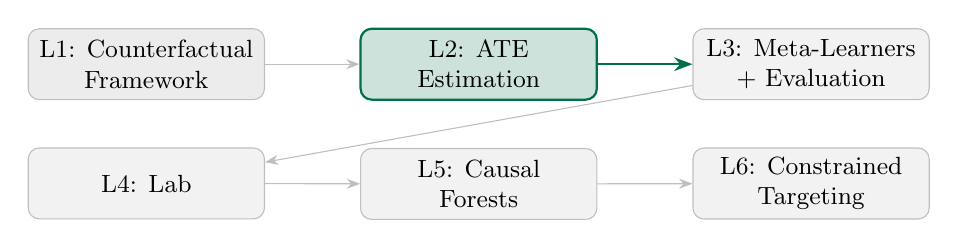
\begin{tikzpicture}[
    node distance=0.6cm and 1.2cm,
    box/.style={draw, rounded corners, minimum width=3cm, minimum height=0.9cm, font=\small, align=center},
    done/.style={box, fill=gray!15, draw=gray!50},
    active/.style={box, fill=sbgreen!20, draw=sbgreen, thick},
    inactive/.style={box, fill=gray!10, draw=gray!50}
]
\node[done] (L1) {L1: Counterfactual\\Framework};
\node[active, right=of L1] (L2) {L2: ATE\\Estimation};
\node[inactive, right=of L2] (L3) {L3: Meta-Learners\\+ Evaluation};
\node[inactive, below=of L1] (L4) {L4: Lab};
\node[inactive, below=of L2] (L5) {L5: Causal\\Forests};
\node[inactive, below=of L3] (L6) {L6: Constrained\\Targeting};

\draw[-{Stealth}, gray!50] (L1) -- (L2);
\draw[-{Stealth}, thick, sbgreen] (L2) -- (L3);
\draw[-{Stealth}, gray!50] (L3) -- (L4);
\draw[-{Stealth}, gray!50] (L4) -- (L5);
\draw[-{Stealth}, gray!50] (L5) -- (L6);
\end{tikzpicture}
\end{center}
\end{frame}

% ====================================================================
\begin{frame}{Today's Plan}

\textbf{Part I: Formalizing the ATE}
\begin{enumerate}
    \item Setup: SUTVA, consistency, potential outcomes notation
    \item The identification problem: selection bias decomposition
    \item Randomization as the solution
    \item ATT vs.\ ATU under imperfect balance; two senses of ``selection''
    \item Estimation: difference in means, standard error, hypothesis testing
    \item Improving precision with covariates
\end{enumerate}

\bigskip

\textbf{Part II: Why the ATE is Not Enough}
\begin{enumerate}
    \setcounter{enumi}{6}
    \item From ATE to CATE: motivation and definition
    \item Preview of CATE estimation
\end{enumerate}

\bigskip
\textbf{Reading:} Chapters 3 of the textbook.
\end{frame}

% ====================================================================
\section{Setup and Notation}
% ====================================================================

\begin{frame}{The Setup}

$n$ customers, indexed $i = 1, \ldots, n$. Each has:

\bigskip

\begin{tabular}{ll}
$X_i \in \mathcal{X}$ & pre-treatment covariates (purchase history, tier, demographics) \\[0.5em]
$D_i \in \{0, 1\}$ & treatment assignment ($1$ = coupon) \\[0.5em]
$Y_i(1), Y_i(0)$ & potential outcomes \\[0.5em]
$Y_i$ & observed outcome
\end{tabular}

\bigskip

\begin{block}{SUTVA (Stable Unit Treatment Value Assumption)}
\begin{enumerate}
    \item \textbf{No interference:} $i$'s outcome doesn't depend on $j$'s assignment
    \item \textbf{No hidden versions:} the coupon is the same for everyone
\end{enumerate}
\end{block}

SUTVA makes the notation $Y_i(1)$, $Y_i(0)$ coherent. Without it, we'd need $Y_i(D_1, \ldots, D_n)$.
\end{frame}

% ====================================================================
\begin{frame}{When SUTVA Fails}

\textbf{Example:} Referral bonus experiment.
\begin{itemize}
    \item Treated customer refers a control customer
    \item Control customer's outcome is \emph{contaminated}
    \item $Y_i$ depends on $\mathbf{D}_{-i}$, not just $D_i$
\end{itemize}

\pause

\textbf{Example:} Ride-hailing surge pricing.
\begin{itemize}
    \item Higher price in zone A shifts demand to zone B; and supply to zone A
    \item Zone B outcomes depend on zone A's treatment
\end{itemize}

\pause

\textbf{Example:} Delivery methods (email vs email); UI design and consumer perception

\pause

\bigskip

\begin{alertblock}{Practical Rule}
When SUTVA fails, the difference-in-means estimator is biased \textbf{even with randomization}. Fix: cluster randomization, switchback designs.
\end{alertblock}
\end{frame}

% ====================================================================
\begin{frame}{What Counts as a ``Unit''?}

The unit is defined by the \textbf{level of treatment assignment}:

\bigskip

\begin{center}
\small
\begin{tabular}{lll}
\toprule
\textbf{Design} & \textbf{Unit} & \textbf{SUTVA requires} \\
\midrule
Randomize by customer & Customer & No spillovers across customers \\
Randomize by city-week & City-week & No spillovers across city-weeks \\
Randomize by customer-week & Customer-week & No spillovers across customer-weeks \\
\bottomrule
\end{tabular}
\end{center}

\bigskip

\begin{alertblock}{Common Mistake}
A store-level experiment records transaction-level data ($100{,}000$ rows). But the effective sample size for inference is the number of \textbf{stores} ($\sim$50), not transactions. Aggregate the data or cluster standard errors at the level of assignment.
\end{alertblock}
\end{frame}

% ====================================================================
\begin{frame}{Consistency and Treatment Effects}

Under SUTVA, the \textbf{observed outcome} is:
\[
Y_i = D_i \cdot Y_i(1) + (1 - D_i) \cdot Y_i(0)
\]

\bigskip

\begin{block}{Treatment Effect Estimands}
\begin{align*}
\text{ITE:} \quad & \tau_i = Y_i(1) - Y_i(0) \quad \text{(unobservable)} \\[0.5em]
\text{ATE:} \quad & \tau = \E[Y(1) - Y(0)] = \E[Y(1)] - \E[Y(0)]
\end{align*}
\end{block}

\bigskip

The ITE is the ideal target; the ATE is what we can estimate.
\end{frame}

% ====================================================================
\begin{frame}{Running Example: Starbucks Coupons}

Two customer types: senior executives ($X = 1$) and junior analysts ($X = 0$), each 50\%.

\bigskip

\begin{center}
\begin{tabular}{lccc}
\toprule
\textbf{Customer type} & $\E[Y(1) \mid X]$ & $\E[Y(0) \mid X]$ & Effect \\
\midrule
Executives ($X = 1$) & 0.80 & 0.75 & $+0.05$ \\
Analysts ($X = 0$) & 0.30 & 0.10 & $+0.20$ \\
\bottomrule
\end{tabular}
\end{center}

\bigskip

$$\tau = 0.5 \times 0.05 + 0.5 \times 0.20 = \mathbf{0.125}$$

\bigskip

Note the heterogeneity: the coupon works much better for analysts.
\end{frame}

% ====================================================================
\section{The Identification Problem}
% ====================================================================

\begin{frame}{Selection Bias Decomposition}

Can we estimate the ATE from observed data?

\[
\E[Y \mid D\!=\!1] - \E[Y \mid D\!=\!0] \stackrel{?}{=} \tau
\]

\pause
\bigskip

\begin{block}{Proposition: Selection Bias Decomposition}
\[
\underbrace{\E[Y \mid D\!=\!1] - \E[Y \mid D\!=\!0]}_{\text{Naive comparison}} = \underbrace{\E[Y(1)\!-\!Y(0) \mid D\!=\!1]}_{\text{ATT}} + \underbrace{\E[Y(0) \mid D\!=\!1] - \E[Y(0) \mid D\!=\!0]}_{\textcolor{warnred}{\text{Selection Bias}}}
\]
\end{block}

\pause
\bigskip

\textbf{Selection bias} $\neq 0$ whenever the treated and untreated would have had different outcomes \emph{even without treatment}.
\end{frame}

% ====================================================================
\begin{frame}{ATT and ATU}

The decomposition introduces the \textbf{Average Treatment Effect on the Treated}:

\[
\tau_{\text{ATT}} = \E[Y(1) - Y(0) \mid D = 1]
\]

The average causal effect among those who \emph{actually received} treatment.

\pause
\bigskip

Its complement is the \textbf{Average Treatment Effect on the Untreated}:

\[
\tau_{\text{ATU}} = \E[Y(1) - Y(0) \mid D = 0]
\]

\pause
\bigskip

The three estimands are linked by the law of total expectation:
\[
\tau = \Prob(D\!=\!1) \cdot \tau_{\text{ATT}} + \Prob(D\!=\!0) \cdot \tau_{\text{ATU}}
\]

When treated and untreated groups differ in composition, ATT and ATU will generally differ from each other and from the ATE.
\end{frame}

% ====================================================================
\begin{frame}{Example 1: Targeting Executives (Overestimate)}

Suppose Starbucks targets coupons at \textbf{executives} (high spenders).

\bigskip

Treated group = 100\% executives; control group = 100\% analysts.

\begin{align*}
\E[Y \mid D = 1] &= \E[Y(1) \mid X = 1] = 0.80 \\
\E[Y \mid D = 0] &= \E[Y(0) \mid X = 0] = 0.10 \\
\text{Naive estimate} &= 0.80 - 0.10 = \textcolor{warnred}{+0.70}
\end{align*}

\pause

Decompose:
\begin{align*}
\underbrace{0.70}_{\text{Naive}} &= \underbrace{0.05}_{\text{ATT}} + \underbrace{0.65}_{\textcolor{warnred}{\text{Selection bias}}}
\end{align*}

Selection bias = $\E[Y(0) \mid D\!=\!1] - \E[Y(0) \mid D\!=\!0] = 0.75 - 0.10 = +0.65$.

\medskip

Executives have higher baseline outcomes. The naive estimate vastly \textbf{overestimates} the causal effect.
\end{frame}

% ====================================================================
\begin{frame}{Example 2: Targeting Analysts (Sign Reversal)}

Now suppose Starbucks targets coupons at \textbf{analysts} (low spenders).

\bigskip

Treated group = 100\% analysts; control group = 100\% executives.

\begin{align*}
\E[Y \mid D = 1] &= \E[Y(1) \mid X = 0] = 0.30 \\
\E[Y \mid D = 0] &= \E[Y(0) \mid X = 1] = 0.75 \\
\text{Naive estimate} &= 0.30 - 0.75 = \textcolor{warnred}{-0.45}
\end{align*}

\pause

Decompose:
\begin{align*}
\underbrace{-0.45}_{\text{Naive}} &= \underbrace{+0.20}_{\text{ATT}} + \underbrace{-0.65}_{\textcolor{warnred}{\text{Selection bias}}}
\end{align*}

Selection bias = $\E[Y(0) \mid D\!=\!1] - \E[Y(0) \mid D\!=\!0] = 0.10 - 0.75 = -0.65$.

\medskip

The coupon appears to \textbf{decrease} purchases by 45 pp, even though the true effect on analysts is $+20$ pp. Selection bias reverses the sign.
\end{frame}

% ====================================================================
\section{Randomization}
% ====================================================================

\begin{frame}{Randomization as the Solution}

\begin{block}{Random Assignment}
\[
D \indep \bigl(Y(0),\, Y(1),\, X\bigr), \qquad 0 < \Prob(D = 1) < 1
\]
\end{block}

\pause
\bigskip

\begin{block}{Theorem: Identification of the ATE}
Under SUTVA and random assignment:
\[
\tau = \E[Y(1)] - \E[Y(0)] = \E[Y \mid D = 1] - \E[Y \mid D = 0]
\]
\end{block}

\textbf{Proof sketch:}
\begin{itemize}
    \item By consistency: $\E[Y \mid D\!=\!1] = \E[Y(1) \mid D\!=\!1]$
    \item By independence: $\E[Y(1) \mid D\!=\!1] = \E[Y(1)]$
    \item Analogously for $D = 0$. Selection bias = 0. $\square$
\end{itemize}
\end{frame}

% ====================================================================
\begin{frame}{Verifying with the Starbucks Example}

Under random 50/50 assignment, each group has 50\% executives, 50\% analysts:

\begin{align*}
\E[Y \mid D = 1] &= 0.5 \times 0.80 + 0.5 \times 0.30 = 0.55 \\
\E[Y \mid D = 0] &= 0.5 \times 0.75 + 0.5 \times 0.10 = 0.425 \\
\text{Difference} &= 0.55 - 0.425 = \textcolor{sbgreen}{\mathbf{0.125}} = \tau \quad \checkmark
\end{align*}

\bigskip
\pause

\begin{block}{Under Perfect Randomization, All Averages Coincide}
\[
\tau = \tau_{\text{ATT}} = \tau_{\text{ATU}} = 0.125
\]
\end{block}

This is because both groups are representative of the population.
\end{frame}

% ====================================================================
\begin{frame}{Example: Targeting Loyal Customers}

The marketing team selects 600 loyal customers for a coupon campaign: 400 executives, 200 analysts. Within this group, they run a proper 50/50 RCT.

\bigskip

\begin{center}
\small
\begin{tabular}{lcccc}
\toprule
& \textbf{Targeted} & \textbf{Treated} & \textbf{Control} & \textbf{Full population} \\
\midrule
Executives & 400 (67\%) & 200 & 200 & 500 (50\%) \\
Analysts & 200 (33\%) & 100 & 100 & 500 (50\%) \\
\bottomrule
\end{tabular}
\end{center}

\pause
\bigskip

Randomization is valid within the targeted group, so the difference-in-means correctly estimates:
\[
\tau_{\text{ATT}} = \tfrac{2}{3} \times 0.05 + \tfrac{1}{3} \times 0.20 = 0.10
\]

But the full-population ATE is $\tau = 0.50 \times 0.05 + 0.50 \times 0.20 = 0.125$.

\bigskip

$\tau_{\text{ATT}} < \tau$ because the targeted group over-represents executives, who benefit less from the coupon. \textbf{Internal validity is fine; external validity is not.}
\end{frame}

% ====================================================================
\begin{frame}{Example: Targeting Lapsing Customers}

Now the team selects 600 lapsing customers: 200 executives, 400 analysts. Again, a proper 50/50 RCT within this group.

\begin{center}
\small
\begin{tabular}{lcccc}
\toprule
& \textbf{Targeted} & \textbf{Treated} & \textbf{Control} & \textbf{Full population} \\
\midrule
Executives & 200 (33\%) & 100 & 100 & 500 (50\%) \\
Analysts & 400 (67\%) & 200 & 200 & 500 (50\%) \\
\bottomrule
\end{tabular}
\end{center}

\pause

Again, randomization is valid within the targeted group:
\[
\tau_{\text{ATT}} = \tfrac{1}{3} \times 0.05 + \tfrac{2}{3} \times 0.20 = 0.15
\]

Now $\tau_{\text{ATT}} > \tau = 0.125$ because the targeted group over-represents analysts, who benefit more.


\begin{alertblock}{Lesson}
Both experiments are internally valid. But the estimated ATT depends on \emph{who was targeted}. Generalizing ATT to the full customer base requires knowing how the targeted population differs from the full population.
\end{alertblock}
\end{frame}

% ====================================================================
\begin{frame}{Two Senses of ``Selection''}

\begin{block}{1. Selection Bias (Internal Validity)}
Treated and control groups differ in baseline outcomes:
\[
\E[Y(0) \mid D = 1] \neq \E[Y(0) \mid D = 0]
\]
The naive comparison does not recover \emph{any} causal effect. This is an \textbf{identification} failure.

Fix: randomization ensures $D \indep (Y(0), Y(1))$, zeroing out the bias term.
\end{block}

\pause

\begin{block}{2. Selection of the Target Population (External Validity)}
Even with valid randomization, the experiment may not represent the full customer base:
\[
\tau_{\text{ATT}} \neq \tau \quad \text{if the targeted population is not representative}
\]
This is a \textbf{generalization} problem. Targeting loyal customers gave ATT $= 0.10 < \tau$.

Fix: reweighting, or recognizing which estimand matches the business decision.
\end{block}
\end{frame}

% ====================================================================
\section{Estimation and Inference}
% ====================================================================

\begin{frame}{The Difference-in-Means Estimator}

Given $n_1$ treated and $n_0$ control:

\[
\hat{\tau} = \bar{Y}_1 - \bar{Y}_0 = \frac{1}{n_1}\sum_{i: D_i = 1} Y_i - \frac{1}{n_0}\sum_{i: D_i = 0} Y_i
\]

\bigskip

Under randomization: $\E[\hat{\tau}] = \tau$ (unbiased).

\bigskip
\pause

\textbf{Standard error:}
\[
\Var(\hat{\tau}) = \frac{\sigma_1^2}{n_1} + \frac{\sigma_0^2}{n_0}
\]

Estimated by plugging in sample variances:
\[
\widehat{\SE}(\hat{\tau}) = \sqrt{\frac{\hat{p}_1(1-\hat{p}_1)}{n_1} + \frac{\hat{p}_0(1-\hat{p}_0)}{n_0}}
\]

For continuous outcomes, replace $\hat{p}(1-\hat{p})$ with $s^2$ in each group.
\end{frame}

% ====================================================================
\begin{frame}{Hypothesis Testing}

\begin{block}{The Test}
\vspace{-0.5em}
\begin{align*}
H_0 : \tau = 0 \quad \text{(coupon has no average effect)} \quad H_1 : \tau \neq 0
\end{align*}
\vspace{-1em}

$z$-statistic: $z = \hat{\tau} \,/\, \widehat{\SE}(\hat{\tau})$. Under $H_0$: $z \approx \mathcal{N}(0,1)$.

\medskip

P-value: $\Prob(|Z| \geq |z|)$. Reject $H_0$ if p-value $< 0.05$.
\end{block}

\pause
\medskip

\textbf{Starbucks example:} $n_1 = n_0 = 500$, $\hat{p}_1 = 0.50$, $\hat{p}_0 = 0.40$.

\begin{align*}
\hat{\tau} &= 0.10, \quad \widehat{\SE} = \sqrt{\frac{0.25}{500} + \frac{0.24}{500}} \approx 0.0313 \\[0.3em]
z &= 0.10 / 0.0313 \approx 3.19, \quad \text{p-value} \approx 0.0014
\end{align*}

95\% CI: $0.10 \pm 1.96 \times 0.0313 = [\,0.039, \; 0.161\,]$
\end{frame}

% ====================================================================
\section{Precision}
% ====================================================================

\begin{frame}{Improving Precision with Covariates}

Under randomization, $\hat{\tau}$ is unbiased with or without covariates.

But covariates can \textbf{reduce variance}:

\[
\Var(\hat{\tau}_{\text{adj}}) \approx (1 - R^2) \cdot \Var(\hat{\tau}_{\text{simple}})
\]

\pause
\bigskip

\textbf{Starbucks example:}

\begin{itemize}
    \item $R^2 \approx 0.43$ (customer type explains 43\% of outcome variance)
    \item SE shrinks: $0.0313 \times \sqrt{0.57} \approx 0.0236$
    \item Confidence interval narrows
\end{itemize}

\bigskip

\begin{alertblock}{Important Distinction}
Covariates improve \emph{precision}, not \emph{validity}. Validity comes from randomization. This is the logic behind CUPED at Netflix and similar methods at tech platforms.
\end{alertblock}
\end{frame}

% ====================================================================
\begin{frame}{Minimum Sample Size}

For a two-sided test at level $\alpha$ with power $1 - \beta$:

\[
n = \frac{(z_{\alpha/2} + z_\beta)^2 \cdot (\sigma_1^2 + \sigma_0^2)}{\tau^2}
\]

\bigskip

\textbf{Example:} Detect $\tau = 0.10$ with 80\% power at $\alpha = 0.05$:

\[
n = \frac{(1.96 + 0.84)^2 \times 0.49}{0.01} = 384 \text{ per group}
\]

\bigskip

With covariate adjustment ($R^2 = 0.43$):

\[
n_{\text{adj}} = 0.57 \times 384 \approx 219 \text{ per group}
\]

A 43\% reduction in required sample size.
\end{frame}

% ====================================================================
\section{The Linear Model}
% ====================================================================

\begin{frame}{The Linear Model View}

Everything we've done has a clean linear model equivalent:

\bigskip

\begin{center}
\small
\begin{tabular}{lll}
\toprule
\textbf{Concept} & \textbf{Potential outcomes} & \textbf{Linear model} \\
\midrule
Basic model & $\tau = \E[Y(1)] - \E[Y(0)]$ & $Y_i = \alpha + \tau D_i + \varepsilon_i$ \\[0.4em]
Selection bias & $\E[Y(0) \mid D\!=\!1] \neq \E[Y(0) \mid D\!=\!0]$ & $\Cov(D_i, \varepsilon_i) \neq 0$ (OVB) \\[0.4em]
Randomization & $D \indep (Y(0), Y(1))$ & $\Cov(D_i, \varepsilon_i) = 0$ \\[0.4em]
Estimation & $\bar{Y}_1 - \bar{Y}_0$ & OLS coefficient on $D$ \\[0.4em]
Covariate adj. & Variance reduction by $1 - R^2$ & ANCOVA: $Y_i = \alpha + \tau D_i + \beta X_i + \varepsilon_i$ \\
\bottomrule
\end{tabular}
\end{center}

\bigskip

Running \texttt{regress Y D} gives numerically identical results to the difference-in-means calculation. The $t$-statistic equals the $z$-statistic.
\end{frame}

% ====================================================================
\begin{frame}{Hidden Confounders and the OVB Formula}

If unobserved $U_i$ affects both $D$ and $Y$:

\[
Y_i = \alpha + \tau D_i + \beta X_i + \gamma U_i + \varepsilon_i
\]

But we estimate without $U$:

\[
\text{Bias} = \gamma \cdot \frac{\Cov(D_i, U_i \mid X_i)}{\Var(D_i \mid X_i)}
\]

\bigskip

\begin{itemize}
    \item $\gamma$: effect of $U$ on $Y$
    \item $\Cov(D, U \mid X)$: how $U$ predicts treatment
    \item Both must be nonzero for bias
    \item No amount of observable controls fixes this
\end{itemize}

\bigskip

\textbf{Randomization zeroes out the bias:} $D \indep U \implies \Cov(D, U) = 0$.
\end{frame}

% ====================================================================
\section{Why ATE Is Not Enough}
% ====================================================================

\begin{frame}{The ATE Can Lose Money}

Send coupons to \textbf{all} 10,000 customers. Margin \textyen 30 per purchase, coupon face value \textyen 10 (cost incurred only when redeemed).

\bigskip

Per person targeted:
\[
\text{Net} = \underbrace{\tau(x) \times 30}_{\text{incremental revenue}} - \underbrace{\E[Y(1) \mid X\!=\!x] \times 10}_{\text{coupon cost on all redeemers}}
\]

\pause
\bigskip

\begin{center}
\begin{tabular}{lcccc}
\toprule
& \textbf{Effect} & \textbf{Redemption rate} & \textbf{Revenue} & \textbf{Net} \\
\midrule
Executives & $+5$ pp & 80\% & \textyen 1.50 & \textcolor{warnred}{$-$\textyen 6.50} \\
Analysts & $+20$ pp & 30\% & \textyen 6.00 & \textcolor{sbgreen}{$+$\textyen 3.00} \\
\bottomrule
\end{tabular}
\end{center}

\pause
\bigskip

Overall: $5{,}000 \times (-6.50) + 5{,}000 \times 3.00 = \textcolor{warnred}{-\text{\textyen}\,17{,}500}$.

\medskip

Executives redeem at high rates but gain little from the coupon. Most of the \textyen 10 subsidy goes to purchases they would have made anyway. \textbf{Targeting only analysts would be profitable.}
\end{frame}

% ====================================================================
\begin{frame}{The CATE: Definition}

\begin{block}{Conditional Average Treatment Effect (CATE)}
\[
\tau(x) = \E[Y(1) - Y(0) \mid X = x] = \E[Y(1) \mid X = x] - \E[Y(0) \mid X = x]
\]
\end{block}

The CATE is a \textbf{function}, not a single number. The ATE is its average:

\[
\tau = \E[\tau(X)]
\]

\pause
\bigskip

\textbf{Identification under randomization:}
\[
\tau(x) = \E[Y \mid D = 1, X = x] - \E[Y \mid D = 0, X = x]
\]

This means: within each subgroup defined by $X = x$, the difference in means estimates the CATE.
\end{frame}

% ====================================================================
\begin{frame}{Starbucks CATEs}

\begin{align*}
\tau(\text{exec}) &= \E[Y \mid D\!=\!1, X\!=\!1] - \E[Y \mid D\!=\!0, X\!=\!1] = 0.80 - 0.75 = 0.05 \\
\tau(\text{analyst}) &= \E[Y \mid D\!=\!1, X\!=\!0] - \E[Y \mid D\!=\!0, X\!=\!0] = 0.30 - 0.10 = 0.20
\end{align*}

Check: $\tau = 0.5 \times 0.05 + 0.5 \times 0.20 = 0.125$ $\checkmark$

\bigskip
\pause

\textbf{The modeling problem:}
\begin{itemize}
    \item With 2 types: trivial (compute within-group means)
    \item With 10,000 customers and dozens of features: need a model for
\end{itemize}
\[
\mu_1(x) = \E[Y \mid D = 1, X = x], \quad \mu_0(x) = \E[Y \mid D = 0, X = x]
\]
then $\hat{\tau}(x) = \hat{\mu}_1(x) - \hat{\mu}_0(x)$.

\bigskip

\textbf{Next time:} Meta-learners (S-Learner, T-Learner) and how to evaluate them.
\end{frame}

% ====================================================================
\begin{frame}{A Taxonomy of Causal Estimands (Summary)}

Collecting all the estimands we have introduced:

\begin{center}
\begin{tabular}{lll}
\toprule
\textbf{Estimand} & \textbf{Definition} & \textbf{Conditions on} \\
\midrule
ITE & $\tau_i = Y_i(1) - Y_i(0)$ & Individual $i$ \\[0.4em]
ATE & $\tau = \E[Y(1) - Y(0)]$ & Everyone \\[0.4em]
ATT & $\tau_{\text{ATT}} = \E[Y(1) - Y(0) \mid D\!=\!1]$ & The treated \\[0.4em]
ATU & $\tau_{\text{ATU}} = \E[Y(1) - Y(0) \mid D\!=\!0]$ & The untreated \\[0.4em]
CATE & $\tau(x) = \E[Y(1) - Y(0) \mid X\!=\!x]$ & Subgroup $X = x$ \\
\bottomrule
\end{tabular}
\end{center}

\bigskip

Under randomization: $\text{ATE} = \text{ATT} = \text{ATU}$.

\medskip

Always: $\text{ATE} = \E[\tau(X)]$.

\medskip

Always: $\tau = \Prob(D\!=\!1) \cdot \tau_{\text{ATT}} + \Prob(D\!=\!0) \cdot \tau_{\text{ATU}}$.
\end{frame}

% ====================================================================
\begin{frame}{Key Takeaways}

\begin{enumerate}
    \item \textbf{SUTVA} makes potential outcomes well-defined. Violations require different designs.
    
    \medskip
    
    \item \textbf{Selection bias:} naive comparison $=$ ATT $+$ bias. Targeting high-baseline customers overestimates; targeting low-baseline customers can reverse the sign.
    
    \medskip
    
    \item \textbf{Randomization} eliminates selection bias and identifies the ATE.
    
    \medskip
    
    \item \textbf{Two senses of selection:} (1) bias that invalidates estimates (internal validity); (2) non-representativeness that limits generalization (external validity, ATT $\neq$ ATE).
    
    \medskip
    
    \item \textbf{Estimation:} $\hat{\tau} = \bar{Y}_1 - \bar{Y}_0$, with $z = \hat{\tau}/\widehat{\SE}$ for testing.
    
    \medskip
    
    \item \textbf{Covariates} reduce variance by $1 - R^2$, but don't affect validity.
    
    \medskip
    
    \item \textbf{The ATE is not enough} for targeting decisions. The CATE $\tau(x)$ captures heterogeneity.
\end{enumerate}
\end{frame}

\end{document}